%!TEX ROOT=formularioFisica.tex

\section{Elettrostatica}\label{sec:elettrostatica}
L'Elettrostatica studia le cariche elettriche nei corpi e come reagiscono fra di loro.\\
Un concetto fondamentale è quello di \textbf{carica}. La carica (identificata con $Q$) è determinata 
dalla somma di tutte le cariche degli elettroni all'interno di ogni corpo. La sua unità di misura è il 
\emph{Coulomb} ($C$).\\[\baselineskip]
Si noti che nelle seguenti formule, $\varepsilon$ è definito come 
$\varepsilon = \varepsilon_0\varepsilon_r$ dove $\varepsilon_0$ è \hyperref[tab:e0]{la costante
dielettrica nel vuoto} e $\varepsilon_r$ è la costante dielettrica nel mezzo.\\
Per gli esercizi si vada a pagina~\pageref{ex:elettrostatica}.

\subsection{Legge di Coulomb}
Attraverso la legge di Coulomb (da non essere confusa con il teorema di Coulomb) si trova la forza che 
intercorre tra due corpi carichi. Si noti che questa formula può essere usata solo se i corpi sono 
puntiformi e fermi.
\begin{equation*}
F = k_0\frac{Q_1Q_2}{r^2} = \frac{1}{4\pi\varepsilon}\frac{Q_1Q_2}{r^2}
\end{equation*}
\hyperref[tab:k0]{$k_0$}: $9.11\cdot10^9\,\text{N}\cdot\text{m}^2\text{/C}^2$

\subsection{Campo elettrico}
Il campo elettrico è generato da una carica. Esso è un campo vettoriale, ciò significa che ad ogni
suo punto si associa un vettore.\\ 
Verranno ora riportate tutte le formule che permettono di trovare o il modulo o il vettore di un
campo elettrico.

\begin{alignat*}{2}
  E &= k_0\frac{Q}{r^2} & &\text{Solo se puntiforme}\\
  \vec{E} &= \frac{\vec{F}}{q} &\qquad \vec{E} &= \sum\limits_{i=0}^{n} \vec{E}_n\\
  E &= -\frac{\Delta V}{\Delta x} & &
\end{alignat*}
%E &= \frac{\sigma}{2\varepsilon_0} & &\text{Se in un condensatore, si divida solo per } \varepsilon\\
%E &= -\frac{\Delta V}{\Delta x} & & \\
\hyperref[tab:k0]{$k_0$}: $9.11\cdot10^9\,\text{N}\cdot\text{m}^2\text{/C}^2$\\
$\Delta V$: d.d.p\\
$\Delta x$: distanza tra le superfici

\subsubsection{Campo di una superficie piana infinita}
Il campo elettrico può essere uniforme, ovvero a tutti i punti si associa un vettore uguale.
\begin{center}
  \begin{tikzpicture}
    \draw[dashed] (0,0) -- ++(1,0);
    \draw (1,0) -- ++(2,0);
    \draw[dashed] (3,0) -- ++(1,0);
    \draw[-stealth] (2,0.5) -- ++(0,-0.45)
            node[pos=0.5, left]{$\vec{E}$};
    \draw[-stealth] (2,-0.5) -- ++(0,0.45)
            node[pos=0.5, left]{$\vec{E}$};
    \node at (1,0.5){$\sigma < 0$};
    
    \draw[dashed] (0,-2) -- ++(1,0);
    \draw (1,-2) -- ++(2,0);
    \draw[dashed] (3,-2) -- ++(1,0);
    \draw[stealth-] (2,-1.5) -- ++(0,-0.45)
            node[pos=0.5, left]{$\vec{E}$};
    \draw[stealth-] (2,-2.5) -- ++(0,0.45)
            node[pos=0.5, left]{$\vec{E}$};
    \node at (1,-1.5){$\sigma > 0$};
  \end{tikzpicture}
\end{center}
\begin{equation*}
E = \frac{\left\lvert\sigma\right\rvert}{2\epsilon_0}
\end{equation*}
$\sigma$: densità di carica $\left(\frac{Q}{A}\right)$

\subsubsection{Campo elettrico all'interno di un condensatore}
Il campo elettrico è costante in ogni punto all'interno del condensatore. All'esterno è $0$.
\begin{center}
  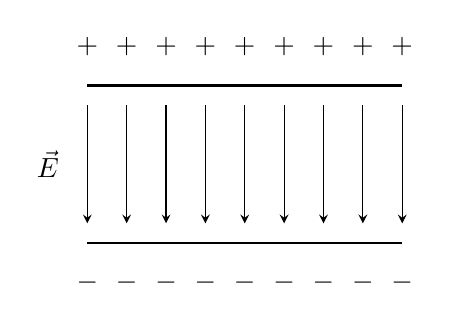
\begin{tikzpicture}
    \draw[thick] (0,0) -- ++(4,0);
    \foreach \ca in {0,0.5,1,...,4}{
      \node at (\ca,0.5){$+$};
      \node at (\ca,-2.5){$-$};
      \draw[-stealth] (\ca,-0.25) -- ++(0,-1.5);
    }
    \draw[thick] (0,-2) -- ++(4,0);
    \node at (-0.5,-1){$\vec{E}$};
  \end{tikzpicture}
\end{center}
\begin{equation*}
E = \frac{\sigma}{\varepsilon}
\end{equation*}
$\sigma$: densità di carica $\left(\frac{Q}{A}\right)$

\subsection{Teorema di Coulomb}
Il teorema di Coulomb definisce il campo elettrico per una qualsiasi superficie.
\begin{equation*}
E = \frac{\sigma}{\epsilon_0}
\end{equation*}

\subsection{Flusso} \label{subsec:flusso}
Il flusso ($\Phi$) è la quantità di campo elettrico ($\vec{E}$), che 
attraversa una superficie ($\vec{S}$).\\
Verranno ora riportate le formule per calcolare il flusso di una superficie.

\begin{alignat*}{2}
  \Phi_S\left(\vec{E}\right) &= \sum\limits_{i=0}^{n}\vec{E}_\cdot\vec{S_i} &\quad &\\
  \Phi_S\left(\vec{E}\right) &= E\cdot S\cos\theta & &\text{Se } S \text{ è piana e } E \text{ 
  uniforme} 
\end{alignat*}
\begin{center}
  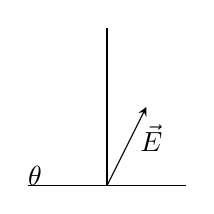
\begin{tikzpicture}
    \coordinate (O) at (1,0);
    \coordinate (A) at (1,2);
    \coordinate (B) at (1.5,1);
    \draw (0,0) -- ++(2,0);
    \draw (O) -- (A);
    \draw[-stealth] (O) -- (B)
      node[pos=0.6,right]{$\vec{E}$};
    \markangle{O}{A}{B}{0.5}{1.4}{$\theta$}
  \end{tikzpicture}
\end{center}

\subsection{Teorema di Gauss}
Il teorema di Gauss definisce il flusso di una superficie \emph{chiusa}.
\begin{equation*}
\Phi_{S_{CH}}\left(\vec{E}\right) = \frac{\sum\limits_{i=0}^{n}Q_i}{\varepsilon}
\end{equation*}

\subsection{Lavoro di un campo elettrico}
Quanto lavoro deve fare un campo elettrico per spostare una carica? Questa sottsezione è dedicata 
proprio a questo.
\begin{equation*}
  L = q\left[V_f - V_i\right]
\end{equation*}
$V_i$: potenziale iniziale\\
$V_f$: potenziale finale\\ [\baselineskip]

Al lavoro sono direttamente collegati \textbf{l'energia potenziale elettrica} ($U$) e 
\textbf{il potenziale elettrico} ($V$). Vengono ora riportate le formule per calcolarle.

\begin{alignat*}{2}
U &= k_0\frac{Q_1Q_2}{r} &\qquad V &= k_0\frac{Q}{r}
\end{alignat*}
\hyperref[tab:k0]{$k_0$}: $9.11\cdot10^9\,\text{N}\cdot\text{m}^2\text{/C}^2$

\subsubsection{Lavoro di una carica in un condensatore}
Il lavoro di una carica è equivalente all'energia interna.
\begin{equation*}
L = \frac{1}{2}QV = \frac{1}{2}QV^2 = \frac{1}{2}\frac{Q^2}{C}
\end{equation*}
$Q$: carica delle pareti\\
$V$: differenza di potenziale\\
$C$: capacità del condensatore

\subsection{Capacità elettrica}\label{sub:elettrostatica:capacita}
La capacità elettrica indica quanta carica può immagazzinare un conduttore isolato. Verranno ora 
riportate le formule per calcolarla.

\begin{alignat*}{2}
C &= \frac{Q}{V} &\qquad &\\
C &= 4\pi\varepsilon & &\text{Specificamente in una sfera isolata}\\
C &= \frac{S\varepsilon}{d} & &\text{Specificamente in un condensatore piano}
\end{alignat*}
Nell'ultima formula, $d$ indica la distanza tra le due armature di un condensatore e $S$ l'area 
delle superfici del condensatore. Un condensatore può essere di qualunque forma o dimensione si
voglia. L'ultima formula è la più generale ci sia.

\subsection{Circuitazione}
La circuitazione ($C$) indica quanta carica passa per una linea chiusa ($\Gamma$).

\begin{equation*}
C_\Gamma\left(\vec{E}\right) = \sum\limits_{i=0}^{n}\vec{E}_i\cdot\vec{l}_i = 
\sum\limits_{i=0}^{n} E_i\cdot l_i\cos\theta
\end{equation*}
$l$: differenza di spostamento\\
Si noti che $theta$ è rispetto alla tangente, non alla normale come nel 
\hyperref[subsec:flusso]{Flusso}.
\begin{center}
  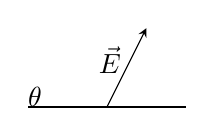
\begin{tikzpicture}
    \coordinate (O) at (1,0);
    \coordinate (A) at (2,0);
    \coordinate (B) at (1.5,1);
    \draw (0,0) -- ++(2,0);
    \draw[-stealth] (O) -- (B)
      node[pos=0.6,left]{$\vec{E}$};
    \markangle{O}{A}{B}{0.5}{1.4}{$\theta$}
  \end{tikzpicture}
\end{center}

\subsection{Dielettrico all'interno di un condensatore}
Come cambia il campo elettrico all'interno di un condensatore se si inserisce un dielettrico?
\begin{equation*}
E_{RIS} = \frac{\sigma-\sigma_p}{\varepsilon}
\end{equation*}

\subsection{Velocità di deriva in un conduttore metallico}
È la velocità media degli elettroni nel conduttore metallico.
\begin{equation*}
  v_d = \frac{i}{n\cdot A\cdot e}
\end{equation*}
\hyperref[tab:e-]{$e^-$}:$-1.60\cdot10^{-19}$ C\\
$n$: numero di elettroni di conduzione\\
$A$: sezione del conduttore\\
$i$: carica massima

